\chapter{Fully connected layers}
As discussed above the Deep Q--Learning had many problems and we were unable to make any significant progress as the simulation times were long, which made parameter searches difficult.
To reduce complexity we decided to start completely from scratch and omit the convolution layers and directly use the field representation as input to the fully connected layers.

\section{Our approach and experiments}
As already stated our new network directly uses the field array as input to its fully connected layer.
Similar to the previous approach, a memory is used which is randomly sampled with a small batch size of $75$ for every training step.
This setup is oriented on a general reinforcement learning tutorial with tensorflow~\cite{ReLeTut}.
We stopped using Double DQN to reduce the amount of parameters needed for training.

Without convolution layers, we were able to test with smaller problems.
With for example $4 \times 4$ and $2$ mines and a fully connected network with $2$ hidden layers with $50$ neurons each we achieve win rates of $94.66\%$ on a test set of $5000$ games.
The agent loses in $4.39\%$ of the games, while getting stuck in $0.95\%$.
A game is won in average after about $4.5$ steps, showing that the network is playing efficiently while also displaying the ability to handle different situations.
Necessary to state is that games lost on the first move are removed from testing statistics and are not used during training.
In Figure~\ref{fig:4_4_2_fully} the training progress is displayed.
The games lost at the first move are not added to the memory as they are not useful for training but are still displayed in the training statistics.

\begin{figure}
	\centering
	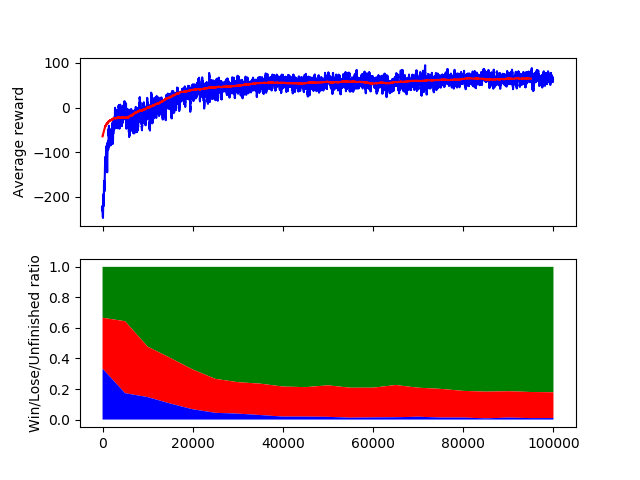
\includegraphics[width=\textwidth]{images/4_4_2_fully.png}
	\caption{Training progress of a $50,50$ fully connected network learning to play on a $4 \times 4$ field with $2$ mines. Win rate is green, red is lose and blue is the unfinished rate averaged over the last $5000$ games. For the average reward blue is averaged over $100$ games and red over $5000$ games.}
	\label{fig:4_4_2_fully}
\end{figure}

Increasing the number of mines also raises the complexity of the game.
Training the agent for $1000000$ games on a $4 \times 4$ field with e.g. $4$ mines results in a win rate of $59.70\%$.
Most of the complexity and thus the decreased win rate lies in the moves needed to win the game.
Winning a game with $4$ mines an average of about $8$ actions are needed.
This is twice the amount 

\begin{figure}
	\centering
	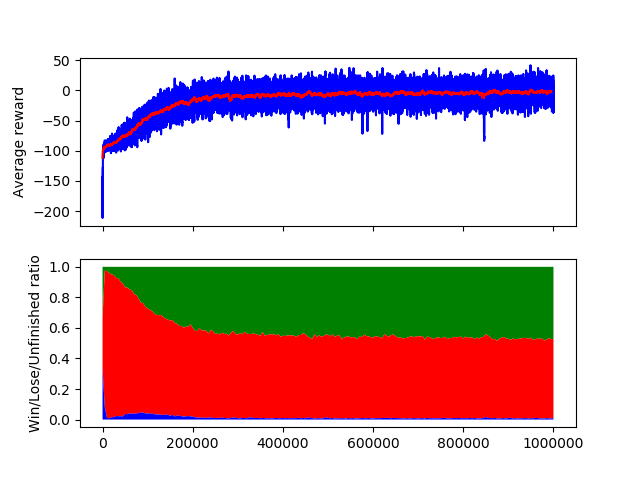
\includegraphics[width=\textwidth]{images/4_4_4_fully.png}
	\caption{Training progress of a $50,50$ fully connected network learning to play on a $4 \times 4$ field with $4$ mines. Win rate is green, red is lose and blue is the unfinished rate averaged over the last $5000$ games. For the average reward blue is averaged over $100$ games and red over $5000$ games.}
	\label{fig:4_4_4_fully}
\end{figure}

As the goal of the project was to play Minesweeper on a `Beginner' level, we increased the size to $5 \times 5$ to see how the pure fully connected network scales with an increased input and action space.
Training the network, progress in Figure~\ref{fig:5_5_5_fully_2million}, needs a lot more games compared to $4 \times 4$.
However after two million games, the agent achieves on $5000$ test games a win rate of $47.78\%$.

\begin{figure}
	\centering
	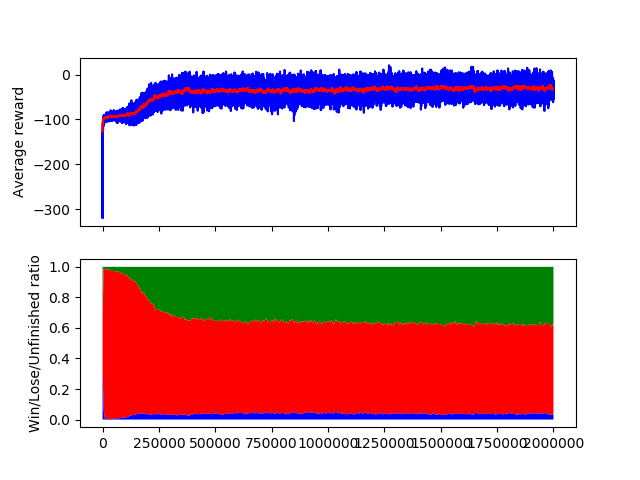
\includegraphics[width=\textwidth]{images/5_5_5_fully_2million.png}
	\caption{Training progress of a $50,50$ fully connected network learning to play on a $5 \times 5$ field with $5$ mines. Win rate is green, red is lose and blue is the unfinished rate averaged over the last $5000$ games. For the average reward blue is averaged over $100$ games and red over $5000$ games.}
	\label{fig:5_5_5_fully_2million}
\end{figure}

As the network topology with $50$ neurons and two layers was just an initial guess, we tried different amounts of neurons and layers to test how it influences the performance.
Two test results are shown in Figure~\ref{fig:layer_test}.
As can be seen, $100$ neurons in one layer are not able to learn Minesweeper as fast as two layers with $50$ neurons each.
Adding a third layer with $50$ neurons increases the complexity of the network resulting in a slower training progress, as can be seen in the bottom of Figure~\ref{fig:layer_test}.
This lead us to choose two fully connected layers for our network.
Doubling the amount of neurons to $100$ on each layer leads to about the same result but increases the computation time.

\begin{figure}
	\centering
	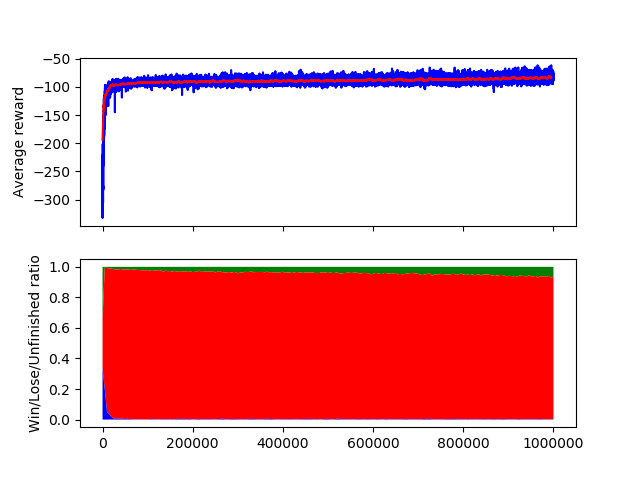
\includegraphics[width=0.8\textwidth]{images/one_layer.png}
	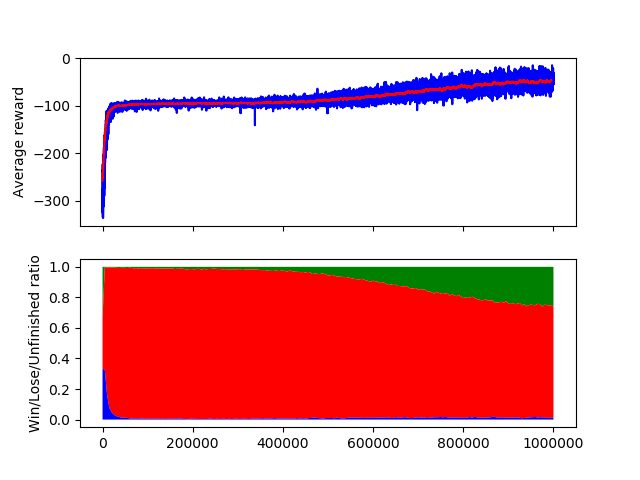
\includegraphics[width=0.8\textwidth]{images/three_layers.png}
	\caption{Training results for one layer network with $100$ neurons (top) and a three layer network with $50$ neurons on each layer. Each network was trained for $1000000$ episodes.}
	\label{fig:layer_test}
\end{figure}

One of the main problems with neural network is the immense amount of parameters needed to be set by the person training the network.
Most of the parameters can not be tested alone but they often interact with other parameters.
This creates dependencies and it is just not possible to evaluate the whole spectrum of possible parameters.
